\subsection{Test of image identification} \label{sec:tests.t1}

The first post-modelling test was a qualitative comparison of the
original arrival-time surfaces and the input spaghetti diagrams given
by the modeller.  This tested first, for correct identification and
location of the lensed images, and second, the correct parities and
ordering for the lensed images in respect of the arrival time.

While we expected the identification of lensed images to be trivial,
given the generally clean appearance of the sims in the test, we
expected the parities and time-ordering to be more difficult.  While
the \spl tutorials had provided some general rules of thumb, to be
consistently correct with the time-ordering, a modeller needs to
develop some intuition for arrival time surfaces.  This is an area
where experience and tutorials training could improve results at a
later stage, and correspondingly, feedback on the difficulties
modellers encounter can help improve the tutorial materials.

\tabref{stats} presents a summary of the test.  The evaluation was
done manually, comparing the input to \spl with the actual
arrival-time surface of the sim.  This amounts to comparing the
upper-left and middle-left panels in each of
Figures~\ref{fig:6941}--\ref{fig:7022}, and similarly the other 111
models.

\begin{table}\centering\begin{tabular}{lr}\hline
    Total & 119 \\
\hline
    errors in image locations  & 9 \\
    errors in image parities or time ordering & 49 \\
\hline
    inaccurate image placement over an arc & 21 \\
    identified two images of four & 5 \\
    identified two nearby images as one & 3 \\
    missed faint images & 1 \\
    proposed too many images & 1 \\
    modelled a three-image arc as one image & 4 \\
    modelled one image as a three-image arc & 5 \\
    swapped minimum and saddle in double  & 2 \\
    swapped minima and saddles in quad & 38 \\
    swapped early and late saddles in a quad & 7 \\
\hline
\end{tabular}
\caption{Table of image-identification errors and the number of models
  containing each.  A model can contain more than one type of error.}
\label{tab:stats}
\end{table}

The images of the system are considered to have been located
correctly, if all the images have been identified and are approximated
within about 5\% of \spl frame used to draw the spaghetti diagram.
That frame size is adjustable by the user, but in practice it is
somewhat larger than the spaghetti diagram.  Such image-placement
errors were found in only 9 models.  That does not include inaccurate
image placement over an arc, which was considered a separate category
of error.

In addition to simple image-placement errors, ten types of errors were
recognised and are listed in \tabref{stats}.  Most of the problems
where due to unclear arc-like structures.  Critical errors like the
failure to identify all five images in a five images system, or to
include too many images, were rare.

The assignment of the parity of the images was a more difficult task,
and was successful in only 60\% of the cases.  The most common error
was swapping of minima and saddle-points in a quad; \figref{7025}
shows an example.  Another, less common, error was flipping the
spaghetti diagram, this swapping the time-ordering of the two saddle
points.

Incorrect image parities and time orderings tended to produce
poorer-looking models, such as the checkboard patterns in the mass map
in \figref{7025}.  Interestingly, however, the enclosed-mass profiles
were quite robust.  We will consider this aspect in the next section.

\FloatBarrier

\begin{figure}
  \centering
  \subfigure{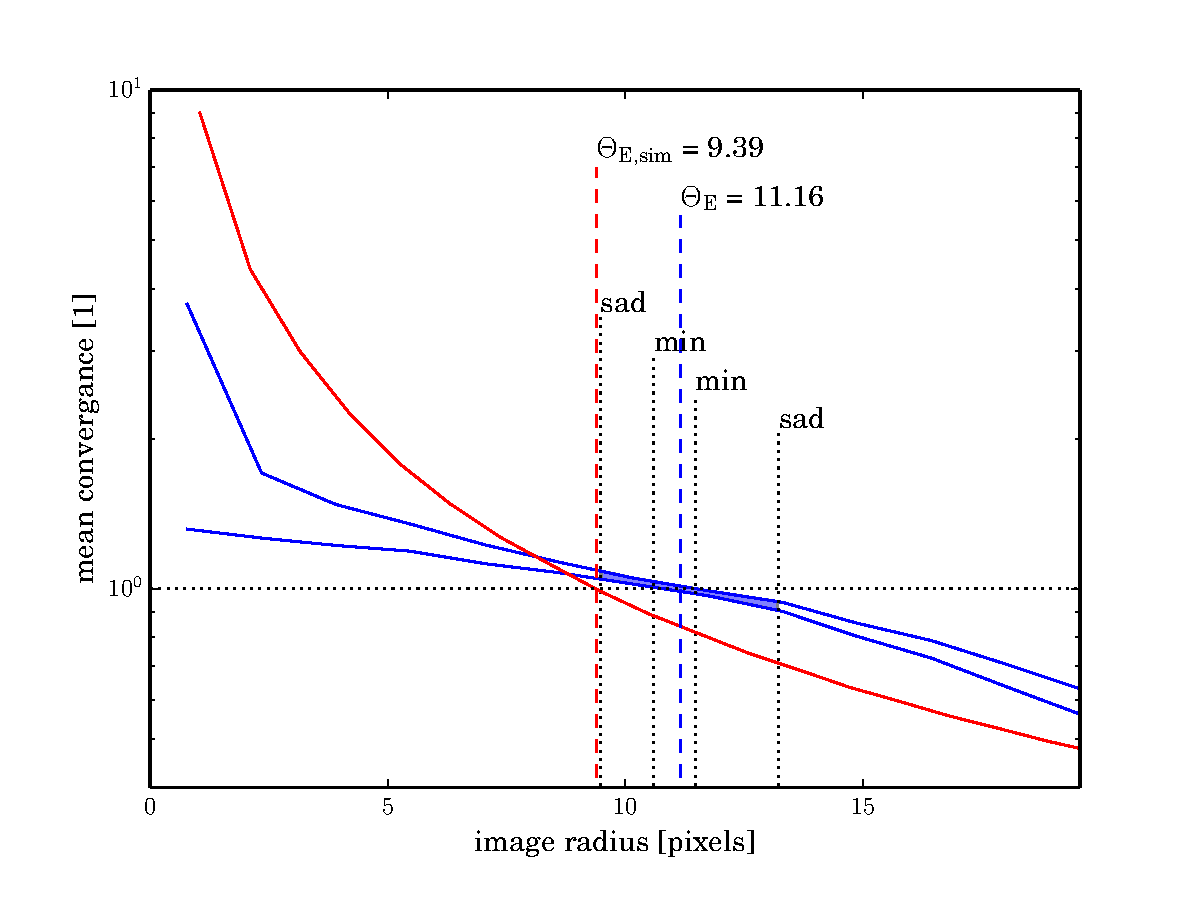
\includegraphics[width=0.8\linewidth]
             {fig/007025_kappa_encl}}
  \subfigure{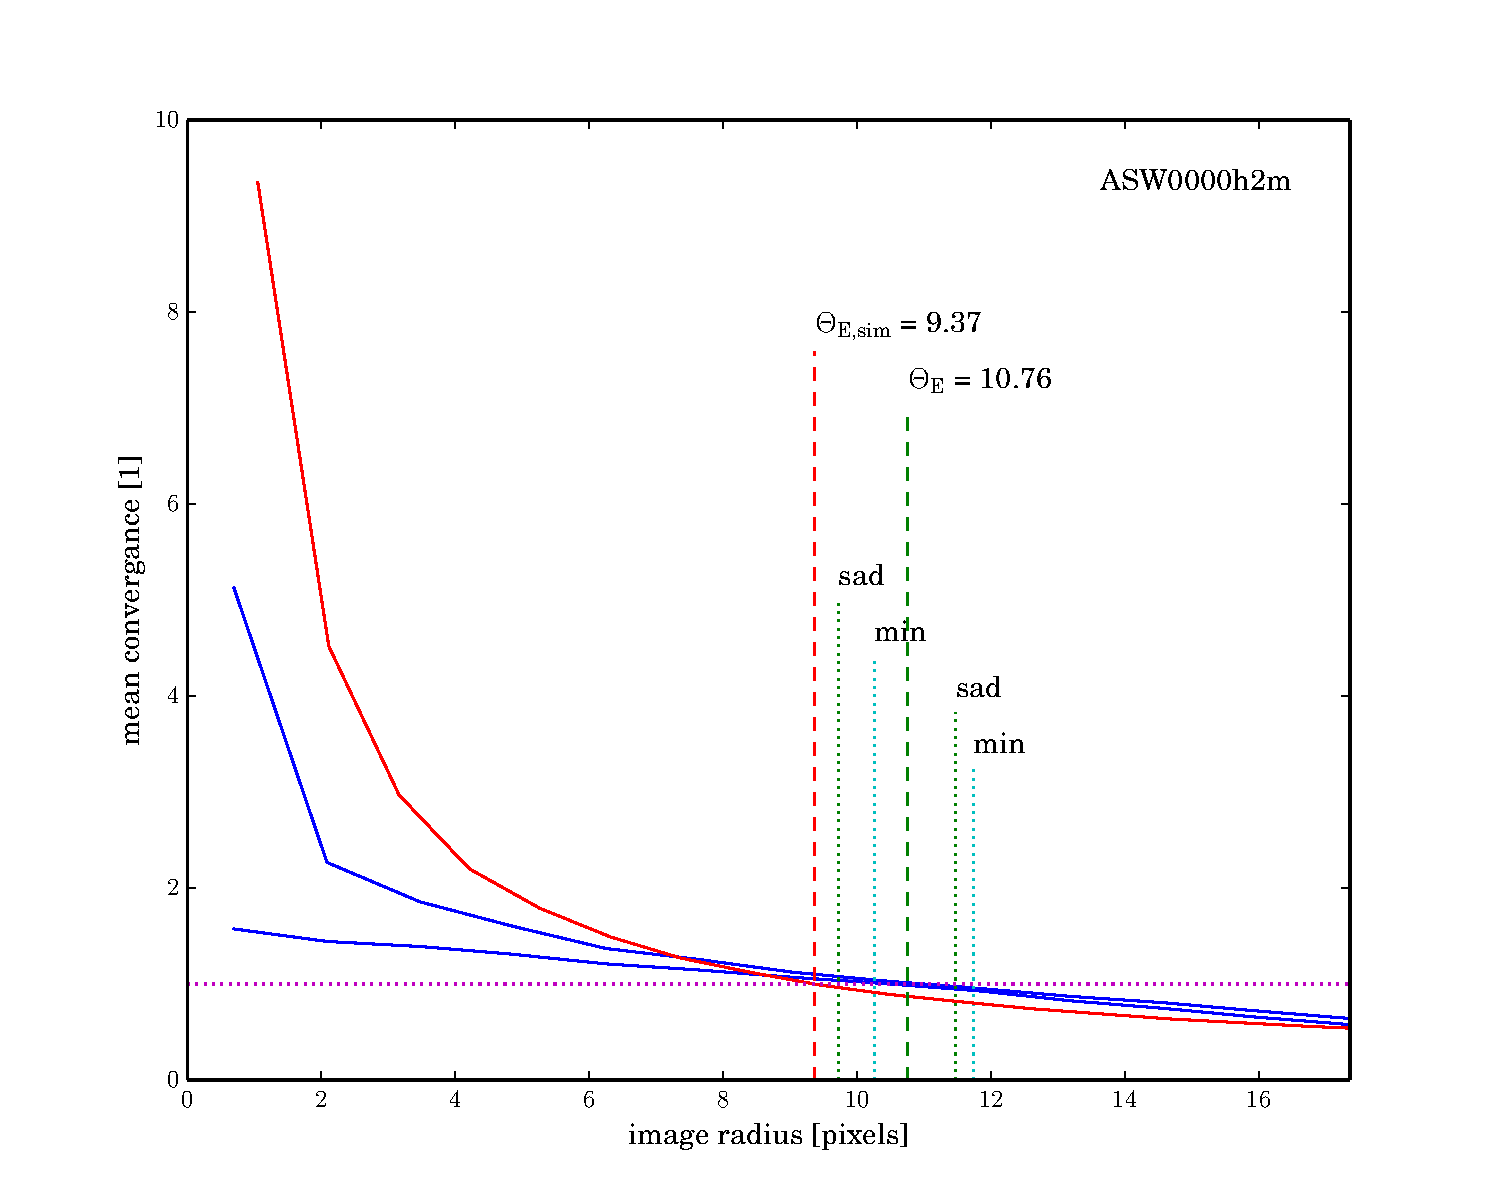
\includegraphics[width=0.8\linewidth]
             {fig/007022_kappa_encl}}
  \subfigure{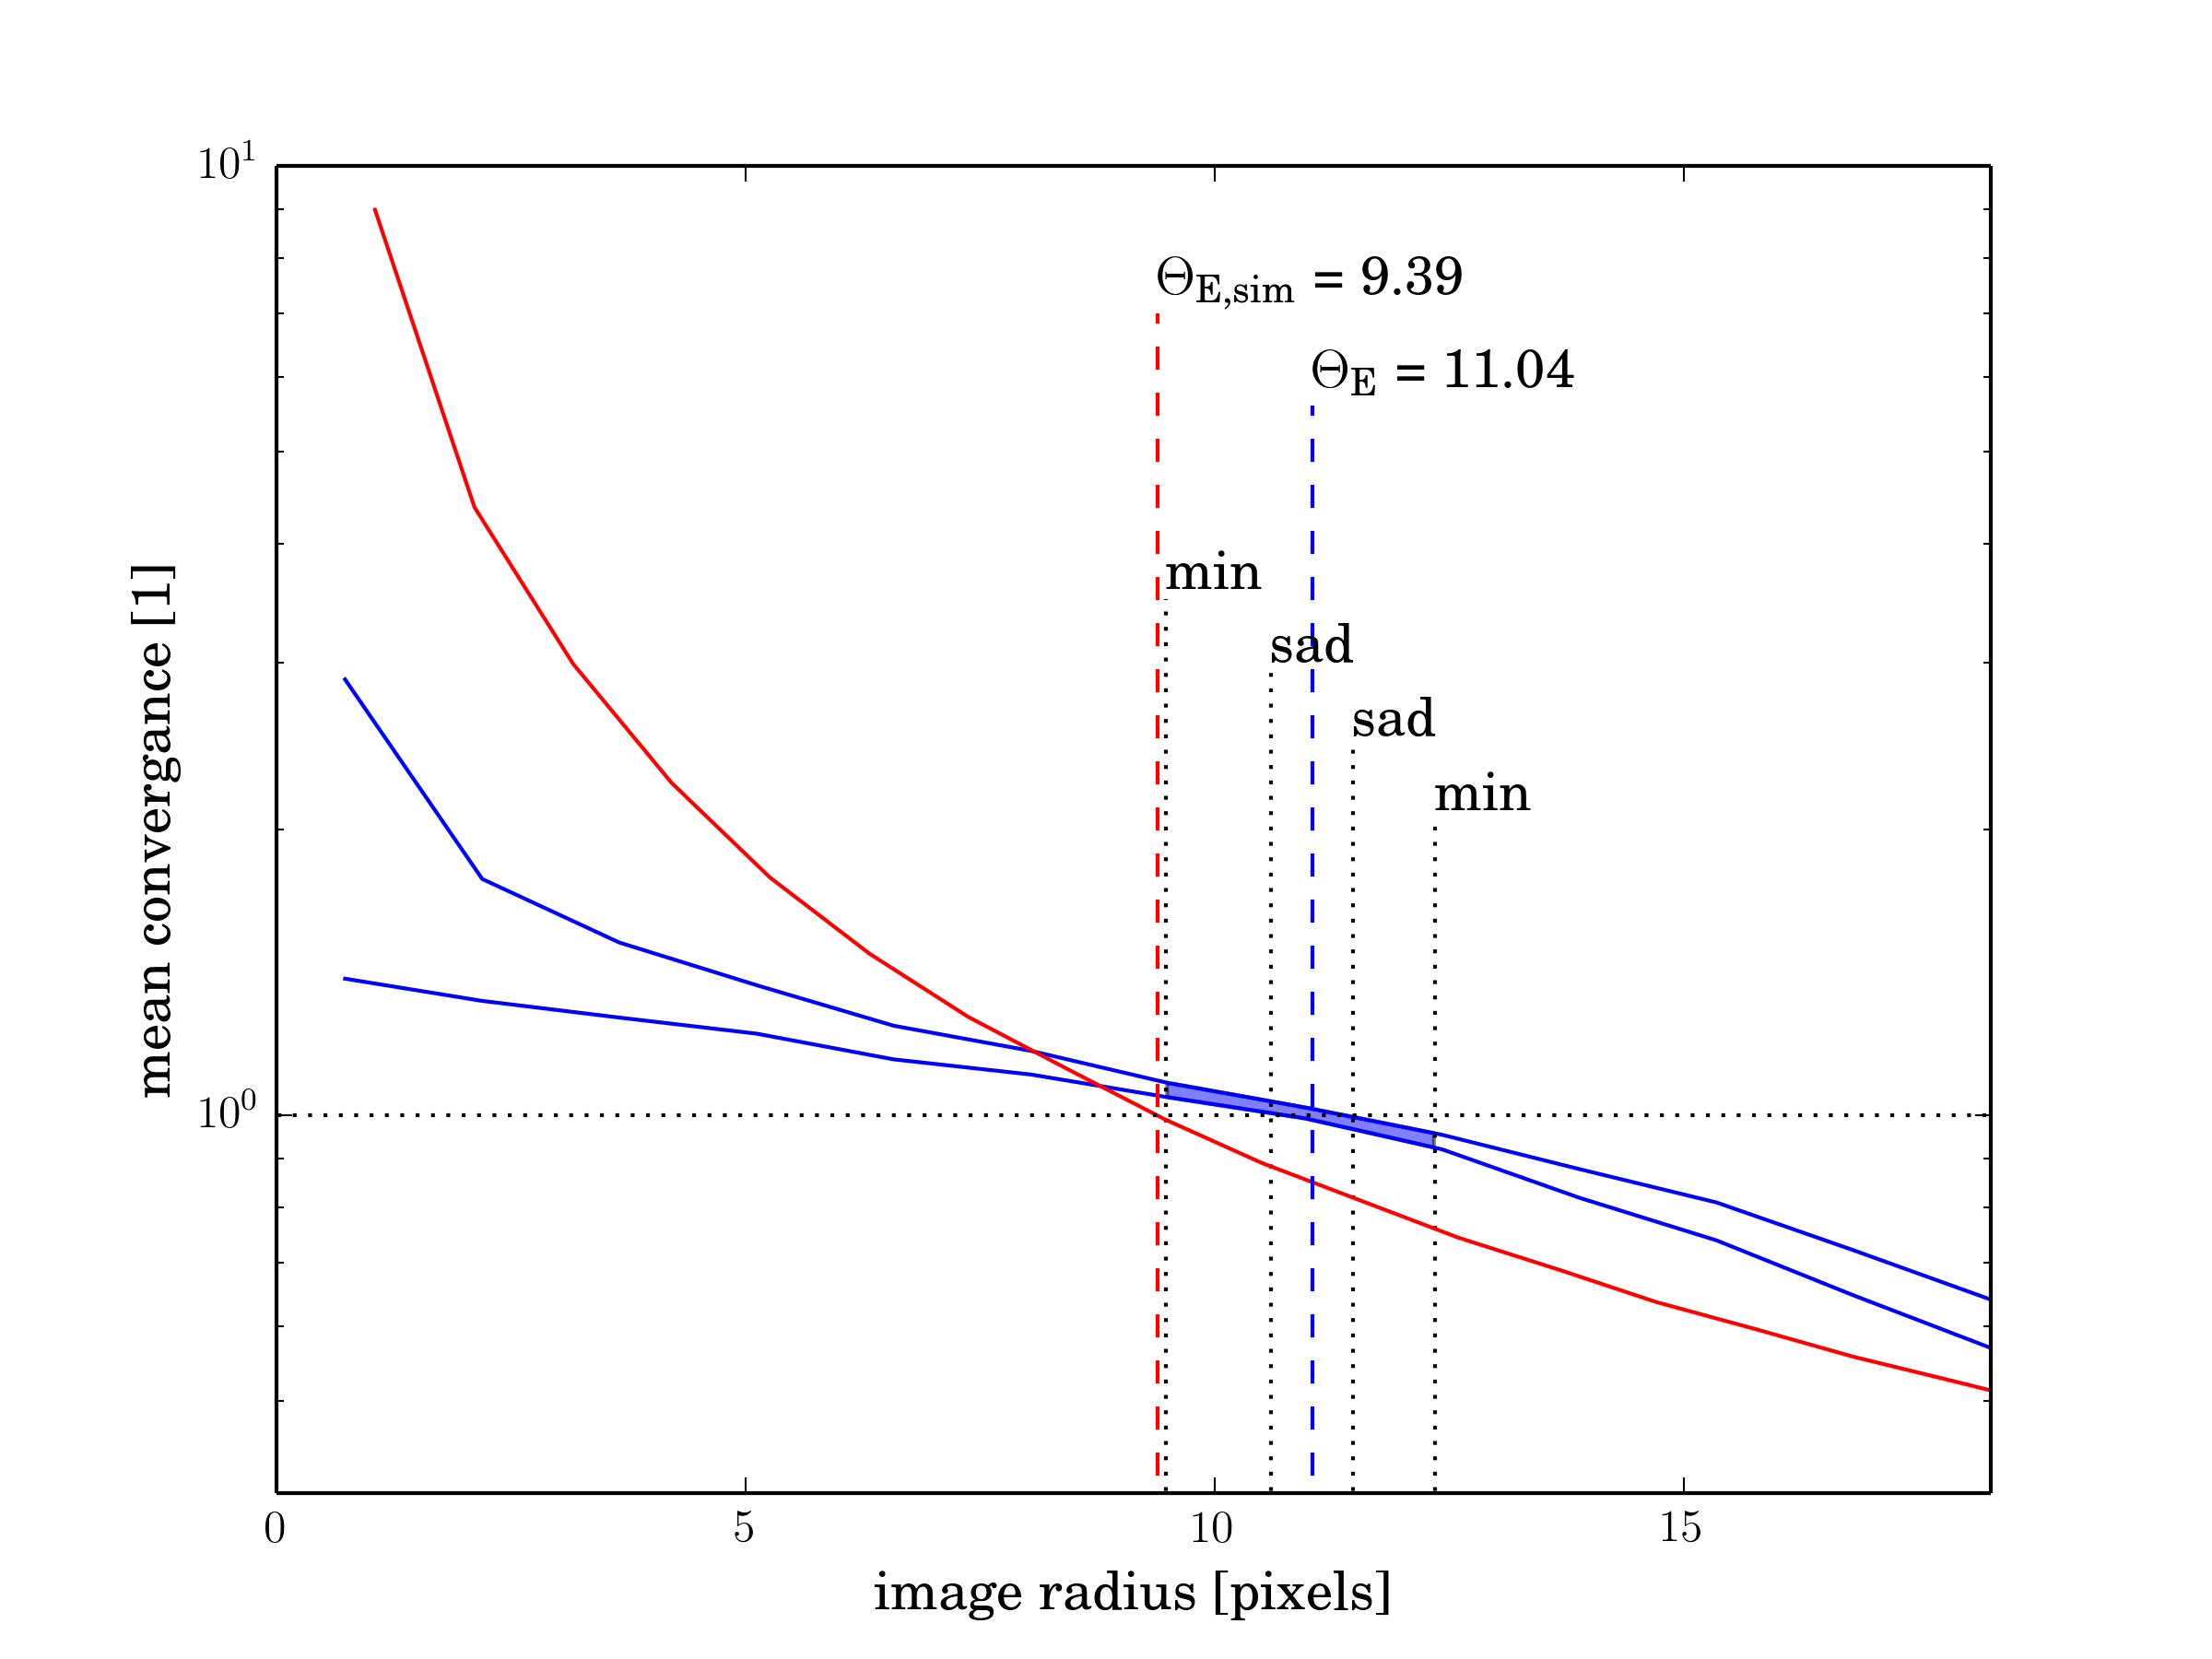
\includegraphics[width=0.8\linewidth]
             {fig/007021_kappa_encl}} \\
  \caption{Mean $\kappa$ inside a circle around the lens centre, as a
    function of the radius of the circle.  (See \secref{tests.t2} for
    details.) The upper panel corresponds to the model shown in
    \figref{7025}, in which the minima and saddle-points have been
    incorrectly swapped.  The middle corresponds to \figref{7022},
    where the image parities were correct.  The lower panel
    corresponds to another model, where the image parities were
    correct but the time-ordering was incorrect.}
\label{fig:kapenc_compare_faulty}
\end{figure}

\subsection{Test of mass-profile recovery} \label{sec:tests.t2}

The second test was to compare the mass distributions $\kappa(x,y)$ of
the sims and of the \spl models.  A visual comparison is presented for
the eight models in Figures~\ref{fig:6941}--\ref{fig:7022}, in the
lower-left versus lower-right panels.  We will summarize the mass
distributions drastically in a single number, the effective Einstein
radius.  Other measures for comparison of free-form lensing mass
distributions appear in \cite{2014arXiv1401.7990C}, but comparing
Einstein radii is already useful.

There is no standard way of defining the Einstein radius of a general
non-circular lens.  We adopt the simple definition
\begin{equation} \label{eq:effRE}
 \langle\kappa\rangle_{\Theta_E} = 1,
\end{equation}
that is, the effective Einstein radius \ERf is such that the
mean $\kappa$ is unity inside a circle of radius \ERf centred at
the lens centre.

To illustrate, \figref{kapenc_compare_faulty} compares the circularly
averaged mass profiles three different models of one particular lens;
two of the models are shown in Figures~\ref{fig:7025} and
\ref{fig:7022}. Each panel in \figref{kapenc_compare_faulty} shows the
mean $\kappa$ within a circle of given radius.  The red curve is the
correct profile for the sim.  The two blue curves are the minimal and
maximal mean enclosed $\kappa$ from the internal ensemble in \spl.
Radial locations of the images are marked, along with the image
parities.  The region between the blue curves is shaded between the
radii of the innermost and the outermost images: this is the
confidence region from the modelling.  The definition (\ref{eq:effRE})
for \ERf corresponds to crossing the dashed horizontal line at
$10^0$: the red curve crosses the dashed line at the actual Einstein
radius \ERf[,act]; the recovered Einstein radius
\ERf[,rec] and its uncertainty are given by the blue curves
crossing the dashed line.  We see that in all three panels, the blue
curves are shallower than the red curve and \ERf[,rec] is
more than \ERf[,act], by more than the model uncertainties.
Now, steeper mass profiles tend to give wider image separations ---
recall that the image separation for a circular isothermal lens is
$2\Theta_E$, whereas for a point mass it is more \citep[see,
  e.g.,][]{2002LNP...608....1C} --- so \ERf[,rec] being too
high is really a consequence of the \spl models being too shallow for
the sims.

\begin{figure*}
  \centering
    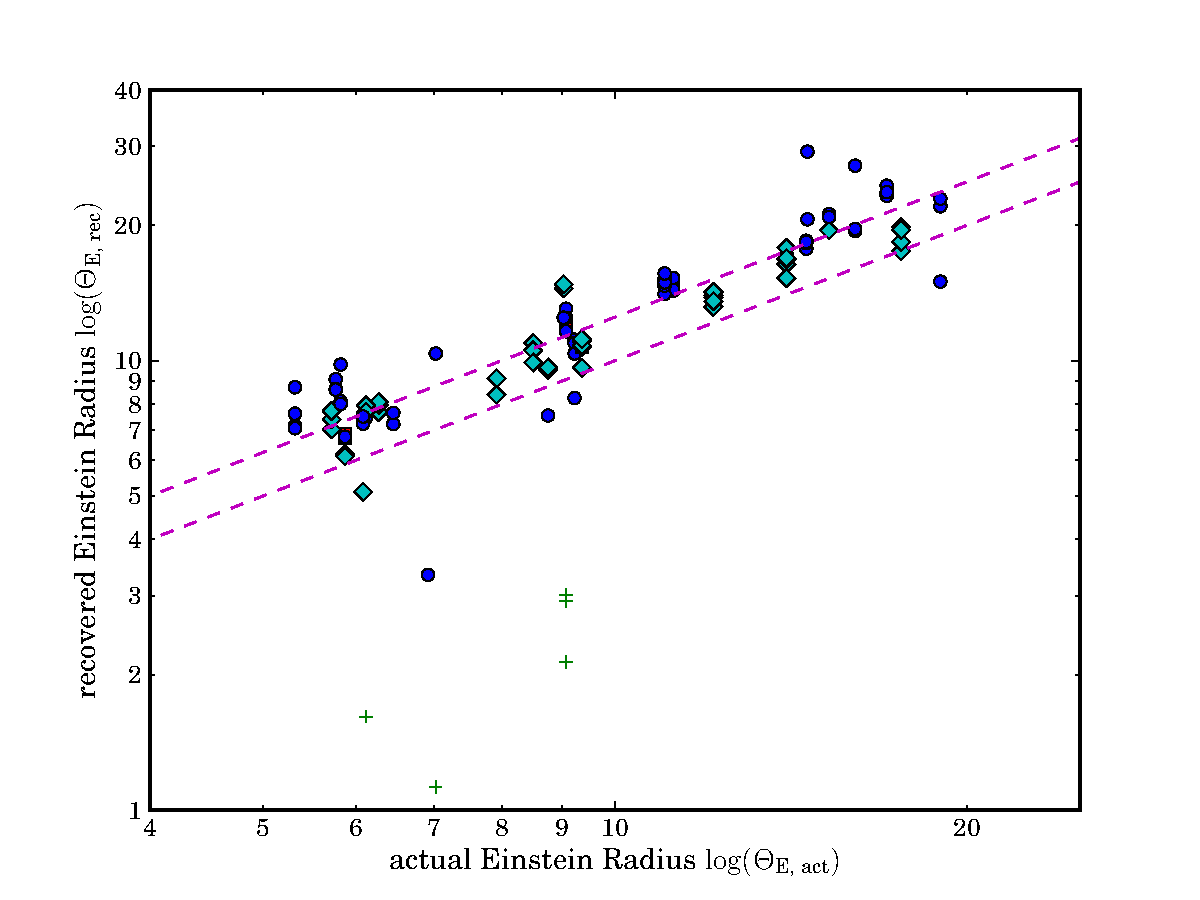
\includegraphics[width=0.90\linewidth]{fig/eR_5}
  \caption{Model-recovered versus actual Einstein radii \ERf[,rec] and
    \ERf[,act].  Circles denote models where the image parities and
    time-orderings were correct, with filled circles for models by an
    expert.  Crosses mark models where the time-ordering was
    incorrect.  Plus signs indicate models flagged by the modeller as
    failures.}
  \label{fig:ER_per_sim}
\end{figure*}

\Figref{ER_per_sim} shows that \ERf[,rec] of the models tend
to be too high.  Discounting the models which were flagged by the
users as poor, the mean and standard deviation of the overestimate are
25\% and 20\%.  The models by an expert (PS) also show a similar bias,
having mean and standard deviation of the overestimate being 20\% and
8\%.  One of the reasons for this is that it is hard to get the center
of the lens on spot.  An offset leads to a flatter mass profile for
the model compared to the simulation.

\section{Outlook} \label{sec:todo}

The lens-modeling challenge indicates that the Spacewarps collective
is good, not only for identifying lens candidates for follow-up, but
modelling candidates as well.

There is, however, plenty of room for improvement.

First, the particular modeling strategy implemented is not the only
one possible.  \spl requires modelers to characterize the overall
image structure in abstract terms based on Fermat's principle, and the
placement of mass distributions is done by the computer.  In other
modeling tools, the user puts down a trial mass distribution and has
the machine refine it.  A few of these modeling programs have also
been designed with citizen science in mind, and would be interesting
in the Spacewarps environment.

Second, \spl needs some enhancements.

\begin{itemize}
\item Currently, \spl does not attempt to model the source shape; the
  user identifies the brightest points on the image, and these are
  taken as images of a point-like source, whose positions must be
  reproduced exactly. For generating a synthetic image, a conical
  source profile is assumed. Fitting for the source profile to
  optimize resemblance to the observed lensed image after the lens
  model has been generated, is algorithmically straightforward
  \citep[cf.][]{2003ApJ...590..673W,2006MNRAS.371..983S} and planned
  to be implemented.  This would alleviate another problem with \spl,
  which is that there is no numerical figure of merit, and assessment
  of a model is a judgment call based on the synthetic image, and on
  whether the mass distribution and the arrival-time surface show
  suspect features.
\item \spl has a tendency to somewhat overestimate the Einstein radius
  (evident from Figure \ref{fig:ER_per_sim}), and it is also apparent
  that the models tend to be too shallow.  This possible explanation
  is that, while the sims are steeply peaked at the centre, the
  pixellated mass model fixes a comparatively large area near the
  central at constant density.  One way to solve this problem would be
  to introduce smaller pixels in the central region, thus enabled a
  steeper centre.
\item Another limitation so far in \spl is that the lens is assumed to
  be dominated by one galaxy, which puts most galaxy-group lenses
  beyond the reach of the modeler. Since complicated group lenses are
  some of the most interesting candidates present, removing this
  limitation is most desirable.  From the users' point of view, it
  would mean that spaghetti contours with more than one maximum can be
  allowed.  For examples, see Figure 5c in \citep{2001ApJ...557..594R}
  and Figure 4b in \cite{2003ApJ...590...39K}.
\item At present, a single false-color composite is used as the data.
  An option could be added to use all available filters, individually
  or in combination, at the user wishes.
\end{itemize}

The third desirable avenue of improvement is to facilitate
collaborative work.

\begin{itemize}
\item As mentioned above, the option of revising an already-archived
  model is already available.  Desired now are tools for comparing
  different models of a given system, both visually and through
  different statistical measures.  As evidenced by a current
  collaborative modeling effort, a particularly interesting candidate
  can lead to an extended discussion and dozens of models.
\item Better tutorial materials are also needed, and this would
  address some of the problem areas found in the modeling challenge.
  For example, we saw in \secref{tests.t1} that volunteers are most
  prone to making errors in two situations: when in identifying an arc-
  like structure while placing the points, and in identifying the
  correct ordering of the points in nearly-symmetric configurations.
\end{itemize}

The \spl program was developed by Kueng, with design suggestions from
Coles, Cornen and Saha, and feedback from all co-authors.  The
simulations were created by A.~More, in consultation with Marshall,
S.~More and Verma.  Modelling was done by Baeten, Cornen, McMillan,
Odermatt, Saha and Wilcox, with post-modelling analysis by Kueng and
Saha.  All authors participated in writing and editing the manuscript.

\section{Acknowledgments}

We thank the Swiss Society for Astrophysics and Astronomy and the
Swiss Academy of Sciences. AV is supported by a research fellowship
from the Leverhulme Trust.

\clearpage

